\documentclass[11pt,a4paper]{article}
%%%%%%%%%%%%%%%%%%%%%%%%% Credit %%%%%%%%%%%%%%%%%%%%%%%%

% template ini dibuat oleh martin.manullang@if.itera.ac.id untuk dipergunakan oleh seluruh sivitas akademik itera.

%%%%%%%%%%%%%%%%%%%%%%%%% PACKAGE starts HERE %%%%%%%%%%%%%%%%%%%%%%%%
\usepackage{graphicx}
\usepackage{caption}
\captionsetup[figure]{name=Gambar}
\usepackage{tabulary}
% \usepackage{amsmath}
\usepackage{fancyhdr}
% \usepackage{amssymb}
% \usepackage{amsthm}
\usepackage{placeins}
% \usepackage{amsfonts}
\usepackage{graphicx}
\usepackage[all]{xy}
\usepackage{tikz}
\usepackage{verbatim}
\usepackage[left=2cm,right=2cm,top=3cm,bottom=2.5cm]{geometry}
\usepackage{hyperref}
\hypersetup{
    colorlinks,
    linkcolor={red!50!black},
    citecolor={blue!50!black},
    urlcolor={blue!80!black}
}
\usepackage{libertine}
\usepackage{libertinust1math}
\usepackage[T1]{fontenc}
\usepackage{inconsolata}

\usepackage{caption}
\usepackage{subcaption}
\usepackage{multirow}
\usepackage{psfrag}
\usepackage[T1]{fontenc}
\usepackage[scaled]{beramono}
% Enable inserting code into the document
\usepackage{listings}
\usepackage{xcolor} 
% custom color & style for listing
\definecolor{codegreen}{rgb}{0,0.6,0}
\definecolor{codegray}{rgb}{0.5,0.5,0.5}
\definecolor{codepurple}{rgb}{0.58,0,0.82}
\definecolor{backcolour}{rgb}{0.95,0.95,0.92}
\lstdefinestyle{mystyle}{
	backgroundcolor=\color{backcolour},   
	commentstyle=\color{green},
	keywordstyle=\color{codegreen},
	numberstyle=\tiny\color{codegray},
	stringstyle=\color{codepurple},
	basicstyle=\ttfamily\footnotesize,
	breakatwhitespace=false,         
	breaklines=true,                 
	captionpos=b,                    
	keepspaces=true,                 
	numbers=left,                    
	numbersep=5pt,                  
	showspaces=false,                
	showstringspaces=false,
	showtabs=false,                  
	tabsize=2
}
\lstset{style=mystyle}
\renewcommand{\lstlistingname}{Kode}
%%%%%%%%%%%%%%%%%%%%%%%%% PACKAGE ends HERE %%%%%%%%%%%%%%%%%%%%%%%%


%%%%%%%%%%%%%%%%%%%%%%%%% Data Diri %%%%%%%%%%%%%%%%%%%%%%%%
\newcommand{\stuid}{120140141}
\newcommand{\student}{\textbf{Bilhaq Avi Dewantara (\stuid{})}}
\newcommand{\course}{\textbf{Sistem Operasi (IF2223)}}
\newcommand{\assignment}{\textbf{03}} % tugas ke...

%%%%%%%%%%%%%%%%%%% using theorem style %%%%%%%%%%%%%%%%%%%%
\newtheorem{thm}{Theorem}
\newtheorem{lem}[thm]{Lemma}
\newtheorem{defn}[thm]{Definition}
\newtheorem{exa}[thm]{Example}
\newtheorem{rem}[thm]{Remark}
\newtheorem{coro}[thm]{Corollary}
\newtheorem{quest}{Question}[section]
%%%%%%%%%%%%%%%%%%%%%%%%%%%%%%%%%%%%%%%%
\usepackage{lipsum}%% a garbage package you don't need except to create examples.
\usepackage{fancyhdr}
\usepackage[ddmmyyyy]{datetime}
\pagestyle{fancy}
\lhead{ \student }
\rhead{ \thepage}
\cfoot{\textbf{Hands On 3: Docker}} % ini untuk judul tugas
\renewcommand{\headrulewidth}{0.4pt}
\renewcommand{\footrulewidth}{0.4pt}

%%%%%%%%%%%%%%  Shortcut for usual set of numbers  %%%%%%%%%%%

\newcommand{\N}{\mathbb{N}}
\newcommand{\Z}{\mathbb{Z}}
\newcommand{\Q}{\mathbb{Q}}
\newcommand{\R}{\mathbb{R}}
\newcommand{\C}{\mathbb{C}}
\setlength\headheight{14pt}

%%%%%%%%%%%%%%%%%%%%%%%%%%%%%%%%%%%%%%%%%%%%%%%%%%%%%%%555

\begin{document}
\thispagestyle{empty}
\begin{center}
	
\includegraphics[scale = 0.15]{Figures/ifitera-header.png}
	\vspace{0.1cm}
\end{center}
% change font family for header section only
%{\fontfamily{LinuxLibertineT-OsF}\large\selectfont 
{\large
\rule{17cm}{0.2cm}\\[0.3cm]
Nama: \student \hfill Tugas Ke: \assignment\\[0.1cm]
Mata Kuliah: \course \hfill Tanggal: \today\\
\rule{17cm}{0.05cm}
\vspace{0.1cm}
}


%%%%%%%%%%%%%%%%%%%%%%%%%%%%%%%%%%%%%%%%%%%%% BODY DOCUMENT %%%%%%%%%%%%%%%%%%%%%%%%%%%%%%%%%%%%%%%%%%%%%
\begin{center}
    \begin{tabular}{ |c|c| }
     \hline
     \multicolumn{2}{|c|}{\textbf{Daftar Anggota Kelompok}} \\
     \hline
     NIM & Nama \\
     \hline
     120140141 & Bilhaq Avi Dewantara \\ 
     120140147 & Gery Melia Suwanda \\ 
     120140150 & Fadhilah Fauza Hamda \\
     \hline
    \end{tabular}
    \end{center}

\section{Tujuan Hands On 3}
    Tujuan adanya tugas Hands On 3 adalah memahami bagaimana cara kerja dari \textit{Docker} ini dan mengimplementasikannya 
    menggunakan \textit{container} layaknya \textit{cloud computing}. Dengan adanya \textit{Docker}, kita dapat melakukan
    pembuatan aplikasi dengan mudah, karena \textit{Docker} sudah terdapat \textit{virtual machine} sebagai pembangan sebuah 
    server. Oleh karena itu, kita tidak perlu membuat sebuah \textit{virtual machine} sendiri untuk men-\textit{deploy} aplikasi 
    ke server. 

\section{Setup Docker}
Pertama yang harus dilakukan dalam Hands On 3 ini adalah mendownload \textit{Docker}. Akan tetapi, hal tersebut tidak bisa 
dijalankan karena diperlukan \textit{Requirements} yang akan dijelaskan sebagai berikut.
\subsection{Requirements (WSL 2)}
    \begin{figure}[h]
        \centering
        \begin{subfigure}[b]{0.4\textwidth}
            \centering
            \def\svgwidth{\columnwidth}
            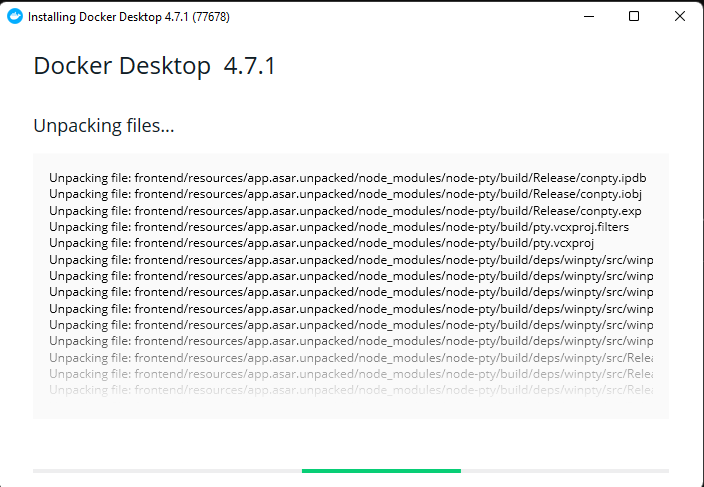
\includegraphics[width=1\textwidth]{Figures/install docker2.png}
            \label{fig:nodeadlock1}
        \end{subfigure}
        \qquad %add desired spacing between images, e. g. ~, \quad, \qquad, \hfill etc. 
        %(or a blank line to force the subfigure onto a new line)
        \begin{subfigure}[b]{0.4\textwidth}
            \centering
            \def\svgwidth{\columnwidth}
            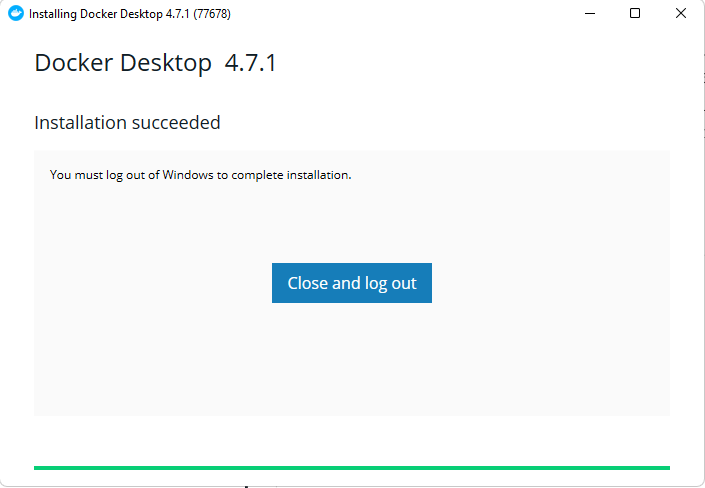
\includegraphics[width=1\textwidth]{Figures/install docker3.png}
            \label{fig:nodeadlock2}
        \end{subfigure}
        \caption{Menginstal Docker}\label{fig:aug}
    \end{figure}

\newpage
    \begin{figure}[h]
    \centering
    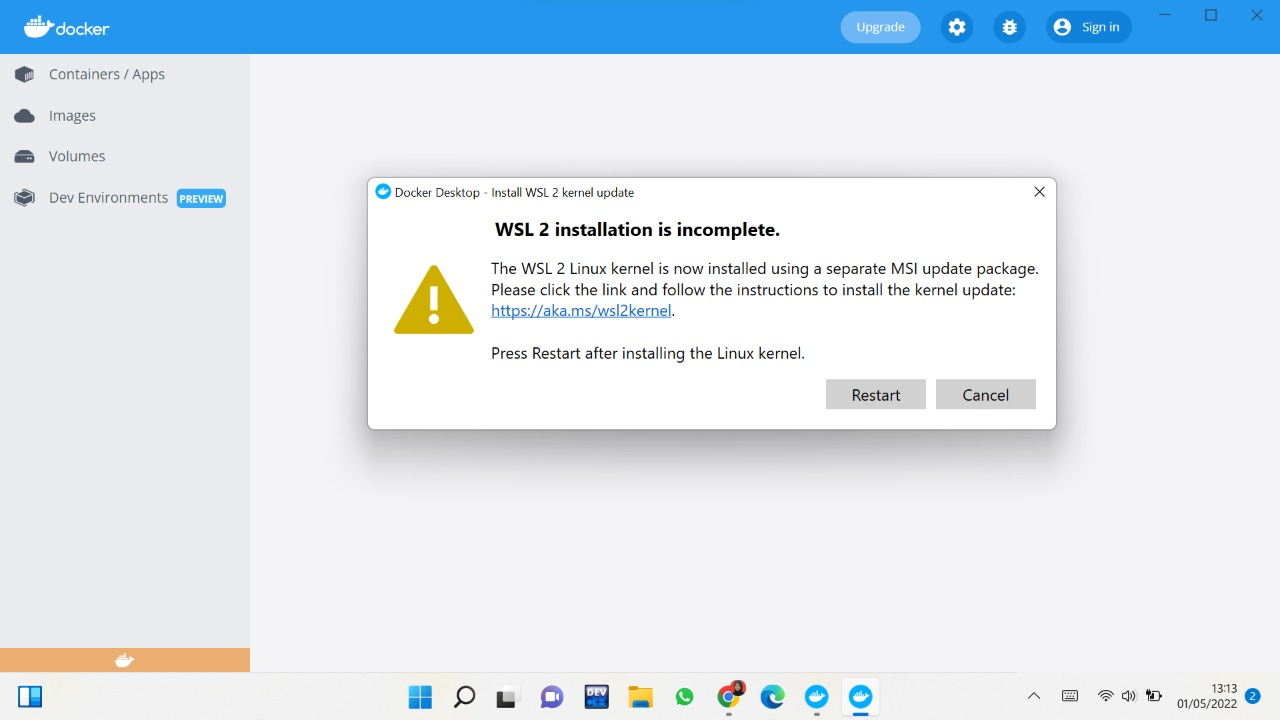
\includegraphics[width = 0.7\textwidth]{Figures/requiremnents_1.png}
    \caption{Pop Up Membutuhkan WSL 2 Untuk Menjalankan Docker}
    \end{figure}

    WSL 2 atau \textit{Windows Subsystem for Linux} adalah sistem operasi yang dikembangkan oleh Microsoft agar sistem operasi Windows
    dapat menjalankan aplikasi yang berbasis \textit{Linux}. Dalam menginstall WSL 2 kita menggunakan Terminal Windows dengan \textit{command} 
    berikut. 
    \begin{lstlisting}[language=bash]
        wsl --install Ubuntu # Menginstall WSL untuk distro Ubuntu
    \end{lstlisting}

    Atau terdapat alternatif lainnya dalam menginstal WSL 2 ini dengan menggunakan \href{https://docs.microsoft.com/en-us/windows/wsl/install-manual#step-1---enable-the-windows-subsystem-for-linux}{Instalasi Manual}
    terlebih dahulu. Berikut merupakan gambar dari Instalasi Manual tersebut dari implementasi step 1 hingga step 5.
    \begin{figure}[h]
        \centering
        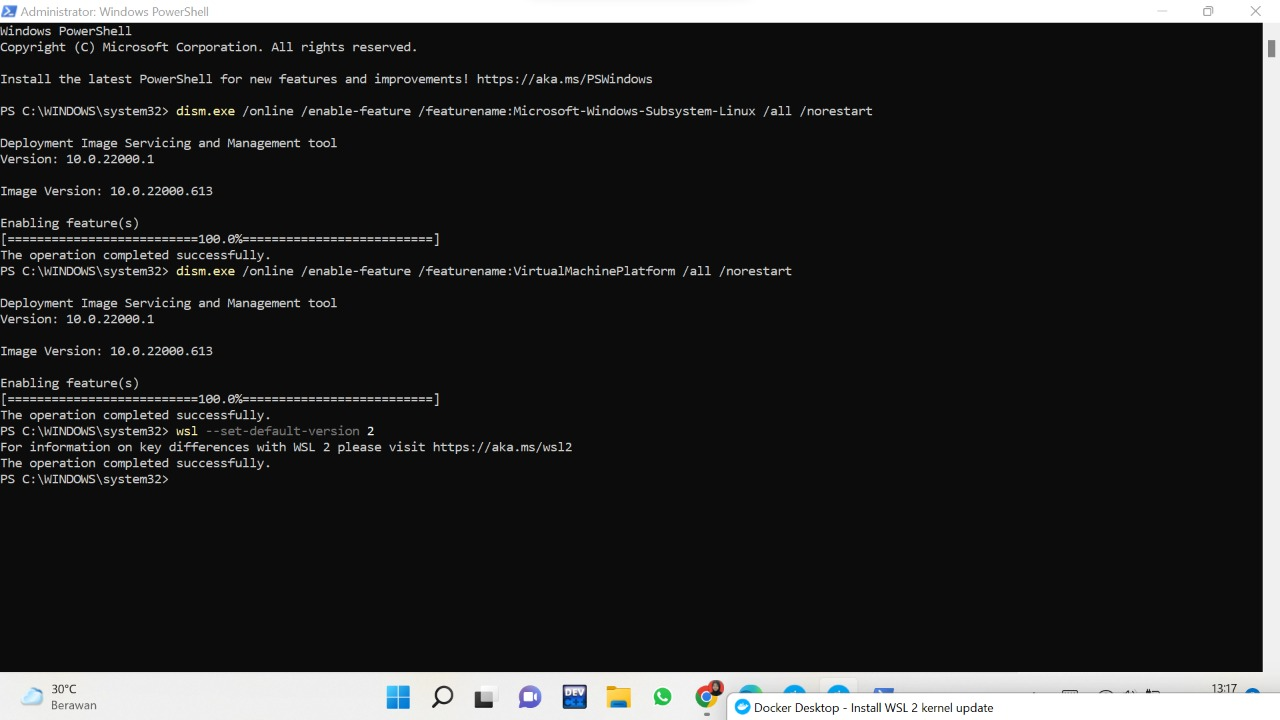
\includegraphics[width = 0.7\textwidth]{Figures/wsl-install_1.png}
        \caption{Instalasi Manual WSL 2 Lewat Terminal Windows}
    \end{figure}

    Setelah di WSL 2 terinstal, maka kita harus me-\textit{restart} PC kita terlebih dahulu. Setelah itu, barulah
    kita bisa membuka aplikasi \textit{Docker} dan untuk mengetahui apakah \textit{Docker} sudah berjalan atau belum 
    ialah dengan melihat statusnya di sebelah bawah bagian kiri aplikasinya. Ketika sudah berwarna hijau maka \textit{Docker} 
    sudah bisa digunakan.
    \begin{figure}[h]
        \centering
        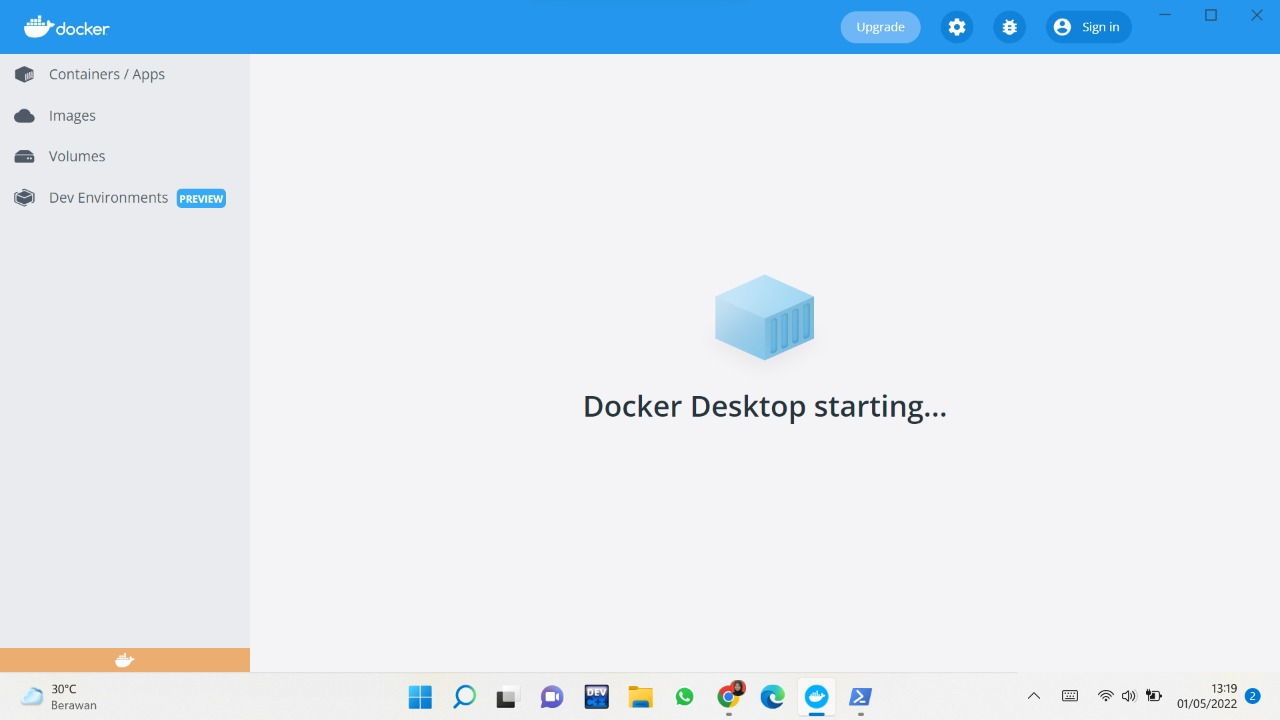
\includegraphics[width = 0.7\textwidth]{Figures/docker-running_1.png}
        \caption{Kondisi Docker Sedang Starting}
    \end{figure}

\newpage
\section{Menjalankan Container Pertama}
\subsection{Hello-World}
    Pada kesempatan ini, kita sudah bisa memulai menjalankan perintah \textit{Docker} dengan menggunakan PowerShell atau CommandPrompt 
    sesuai dengan keinginan \textit{User}. Awal mula yang harus kita coba untuk mengeceknya dengan mengetik perintah berikut pada PowerShell.
    \begin{lstlisting}[language=bash]
        docker run hello-world
    \end{lstlisting}

    \begin{figure}[h]
        \centering
        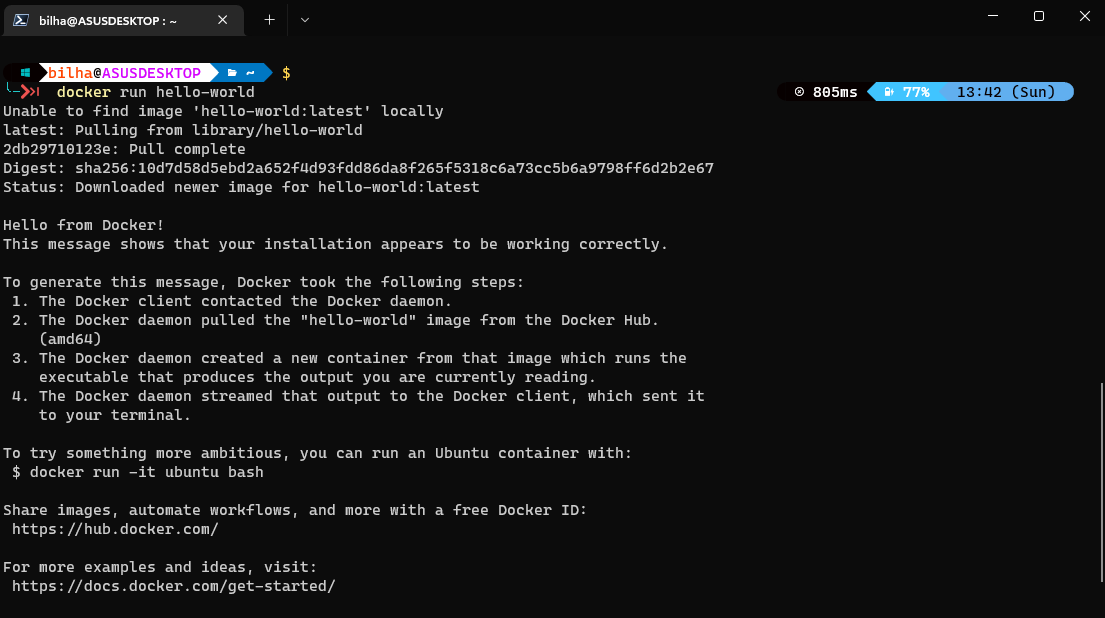
\includegraphics[width = 0.7\textwidth]{Figures/docker-run hello world.png}
        \caption{Docker Run Hello-World}
    \end{figure}

\subsection{Alpine Linux}
    Pada langkah selanjutnya, kita akan mencoba menjalankan \textit{container} dari \textit{Alpine Linux} yang sudah terinstal di PC kita. Perintah yang 
    harus digunakan pada langkah ini ialah melakukan \textit{pull container} dengan perintah sebagai berikut.
    \begin{lstlisting}[language=bash]
        docker pull alpine
    \end{lstlisting}

    \begin{figure}[h]
        \centering
        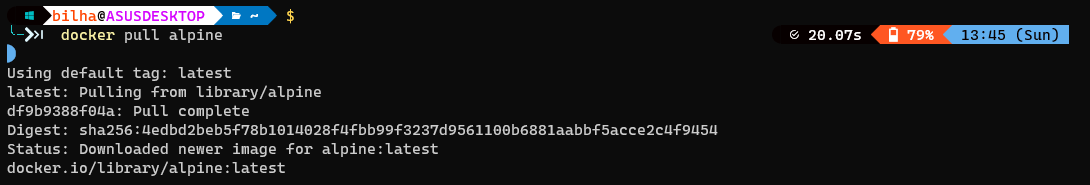
\includegraphics[width = 0.7\textwidth]{Figures/docker-pull_alpine.png}
        \caption{Docker Pull Alpine}
    \end{figure}

\subsubsection{Docker Images}
    Setelah langkah \textit{pull container} berhasil dijalankan, yang mana akan memuat \textit{library/alpine} ke dalam PC lalu disimpan ke dalam sistem 
    yang akan digunakan. Langkah selanjutnya ialah mengecek image apa saja yang sudah pernah kita \textit{pull} atau unduh dengan menggunakan perintah 
    berikut.
    \begin{lstlisting}[language=bash]
        docker images
    \end{lstlisting}

    \begin{figure}[h]
        \centering
        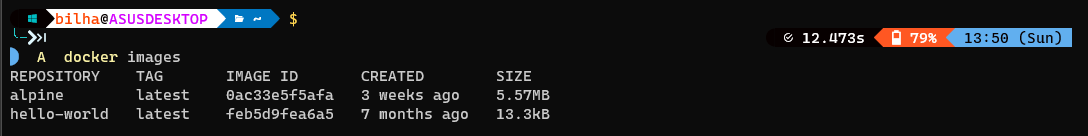
\includegraphics[width = 0.7\textwidth]{Figures/docker-images.png}
        \caption{Docker Images}
    \end{figure}

    Langkah berikutya ialah kita akan memperlihatkan sistem memproses \textit{container} yang
    telah terisolasi. Dalam hal ini, \textit{Container} merupakan sebuah proses yang menjalankan \textit{Host} 
    yang mana \textit{Host} berupa \textit{local}. Saat operator \textit{docker run} di eksekusi, \textit{cotainer} 
    yang sudah dijalankan akan terisolasi akibat mempunyai file sistem dan jaringan sendiri dengan pohon proses 
    yang terpisah dari \textit{Host}. Untuk menjalankan \textit{container docker alpine} dengan urutan \textit{image} ini, 
    kita dapat menggunakan perintah berikut.
    \begin{lstlisting}[language=bash]
        docker run alpine ls -l
    \end{lstlisting}

    \begin{figure}[h]
        \centering
        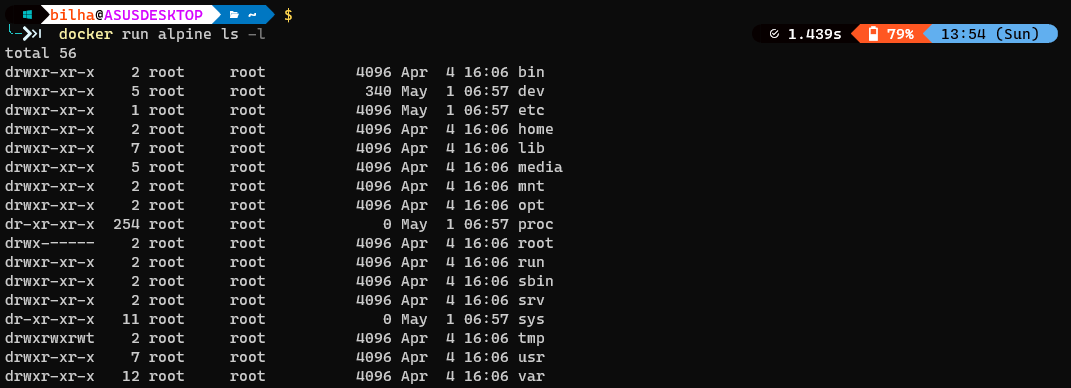
\includegraphics[width = 0.7\textwidth]{Figures/docker-run alpine ls -l.png}
        \caption{Docker Run Alpine ls -l}
    \end{figure}

    Perintah selanjutnya kita akan menampilkan "Hello World" pada Terminal dengan menggunakan perintah 
    \textit{container alpine docker} dan ditambah oleh perintah \textit{echo} yang juga terdapat pada 
    \textit{container alpine}. Untuk perintahnya ialah sebagai berikut.
    \begin{lstlisting}[language=bash]
        docker run alpine echo "Hello World"
    \end{lstlisting}

    \begin{figure}[h]
        \centering
        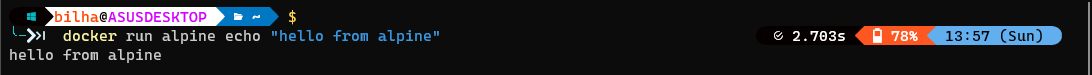
\includegraphics[width = 0.7\textwidth]{Figures/hello_from_alpine.png}
        \caption{Hello World Pada Alpine}
    \end{figure}

    \newpage
    Berikutnya ialah kita mencoba masuk ke dalam \textit{bash} dari \textit{Container Alpine} tersebut dengan menambahkan 
    opsi ketika menjalankan perintah \textit{Cointainer} tersebut. Perintah yang digunakan ialah sebagai berikut.
    \begin{lstlisting}[language=bash]
        docker run -it alpine /bin/sh
    \end{lstlisting}
    \begin{figure}[h]
        \centering
        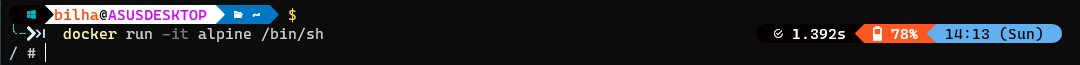
\includegraphics[width = 0.7\textwidth]{Figures/bin-sh.png}
        \caption{Bash dari Container Alpine}
    \end{figure}

    Dari Gambar 10 dapat terlihat bahwa tidak menampilkan \textit{ouput} ke layar, karena hal tersebut hanya 
    mengeluarkan \textit{bash} atau \textit{interactive shells} sesaat perintah di atas dijalankan. Oleh karena itu, 
    diberikanlah \textit{command} atau perintah baru di dalam /bin/sh ini. Perintah yang akan kita berikan untuk menampilkan 
    \textit{list} dari seluruh file yang ada pada /bin/sh ialah sebagai berikut.
    \begin{lstlisting}[language=bash]
        / # ls
    \end{lstlisting}
    \begin{figure}[h]
        \centering
        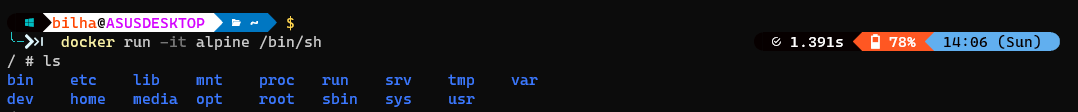
\includegraphics[width = 0.7\textwidth]{Figures/list.png}
        \caption{List dari /bin/sh}
    \end{figure}
    Selanjutnya masih pada \textit{bash} bin/sh, kita akan memberikan perintah untuk menampilkan seluruh informasi dasar 
    yang dimiliki oleh sistem. Perintah yang digunakan ialah sebagai berikut.
    \begin{lstlisting}[language=bash]
        / # uname -a
    \end{lstlisting}
    \begin{figure}[h]
        \centering
        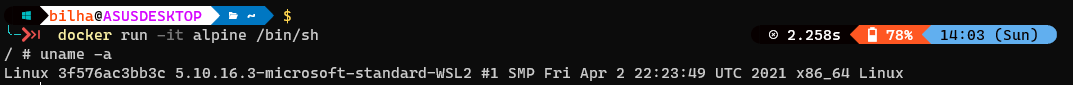
\includegraphics[width = 0.7\textwidth]{Figures/uname -a.png}
        \caption{uname -a dari /bin/sh}
    \end{figure}
    \newpage
    Setelah kedua perintah pada bin/sh ini dijalankan maka kita bisa keluar dari \textit{bash} tersebut dengan perintah.
    \begin{lstlisting}[language=bash]
        / # exit
    \end{lstlisting}
    Pada langkah terakhir yang digunakan untuk menampilkan \textit{container} yang sudah kita jalankan sebelum-sebelumnya 
    dengan menggunakan perintah.
    \begin{lstlisting}[language=bash]
        docker ps -a
    \end{lstlisting}

    \begin{figure}[h]
        \centering
        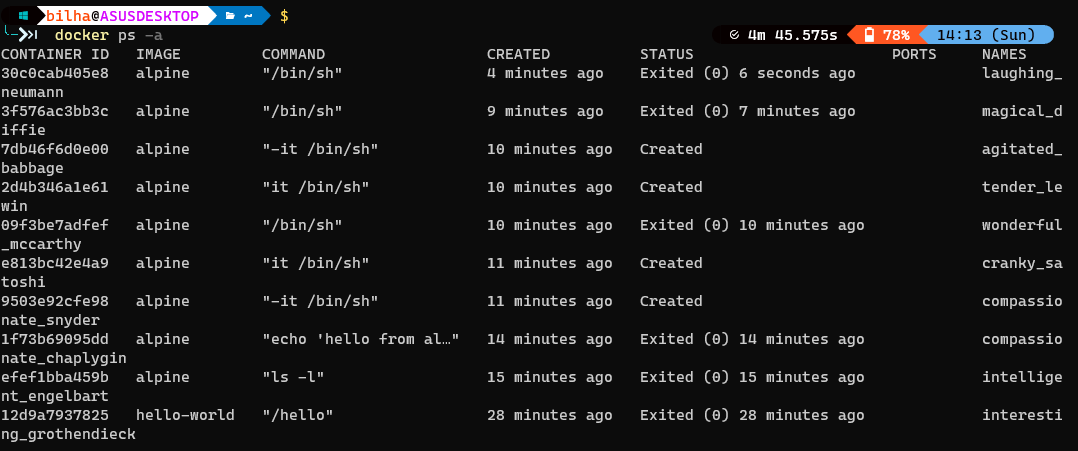
\includegraphics[width = 0.7\textwidth]{Figures/docker ps-a.png}
        \caption{Docker Ps -a}
    \end{figure}

    Faktanya, kita dapat melihat \textit{container} yang telah kita jalankan sebelumnya pada aplikasi \textit{Docker} seperti pada 
    gambar berikut.
    \begin{figure}[h]
        \centering
        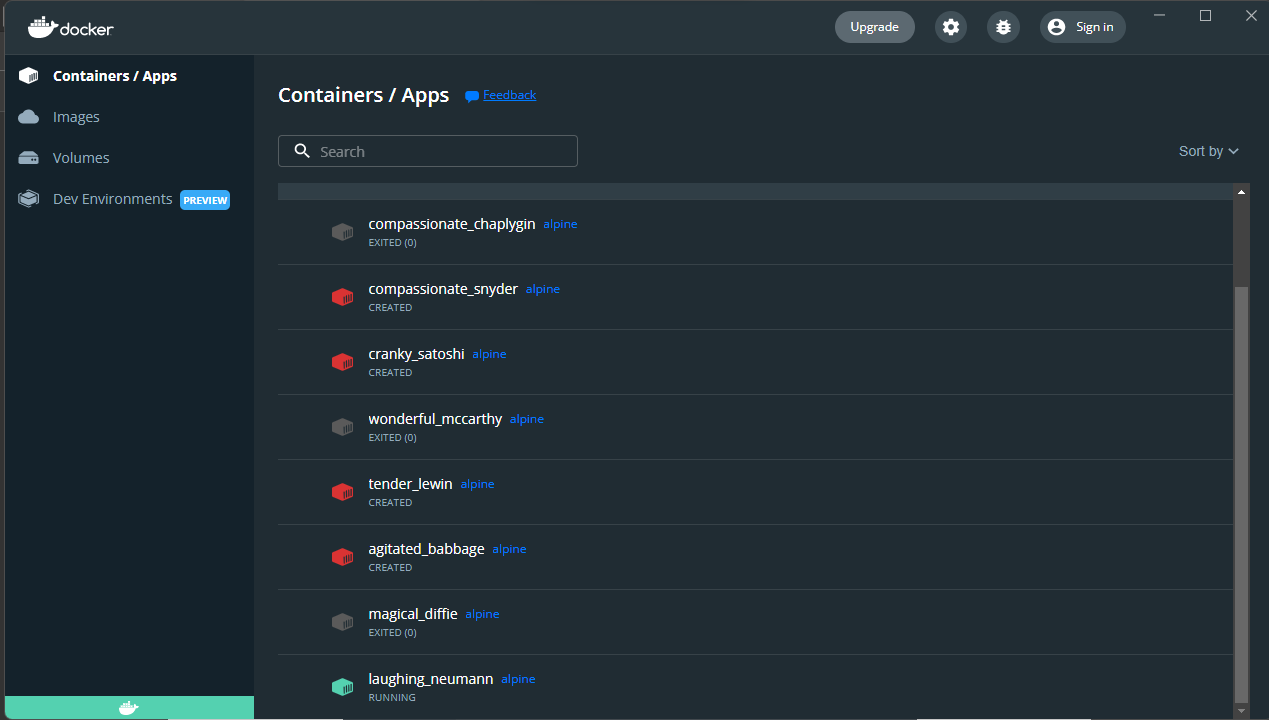
\includegraphics[width = 0.7\textwidth]{Figures/tampilan container.png}
        \caption{\textit{Container} Pada Aplikasi Docker}
    \end{figure}

\section{Pertanyaan Hands On}
\subsection{Apa itu Docker?}
    Docker adalah sebuah aplikasi yang bersifat \textit{opensource} yang memiliki fungsi sebagai wadah atau \textit{container} untuk memasukkan sebuah perangkat lunak 
    secara lengkap beserta semua hal lainnya yang dibutuhkan oleh perangkat lunak tersebut agar dapat berfungsi. Docker \textit{container} ini hampir mirip seperti virtual machine, 
    tetapi dengan sistem yang lebih ringan. Karena sistem \textit{docker} tidak membawa keseluruhan sistem operasi \cite{goasguen_2015}.

\subsection{Apa fungsi dari perintah "docker run"?}
    Perintah \textit{"docker run"} berfungsi dalam menjalankan sebuah \textit{container}. Dengan perintah ini, \textit{docker} akan mencari \textit{image} sesuai dengan letak lokal dari 
    \textit{container} tersebut dan menjalankannya. Apabila pada lokal tidak terdapat \textit{image} yang diminta, maka akan memulai mencarinya di global dan akan melakukan \textit{pull image} 
    tersebut pada lokal. 

\subsection{Apa yang dimaksud dengan \textit{container}?}
    Container adalah wadah yang digunakan untuk mengemas dan menjalankan sebuah aplikasi. Wadah ini sendiri mencakup kode, \textit{runtime}, \textit{system tools}, dan pengaturan. Namun, container hanya dapat 
    mengakses \textit{resource} yang telah ditentukan dalam gambar \textit{docker} saja.

\subsection{Apa yang terjadi ketika perintah "docker ps -a" dilakukan?}
    Perintah \textit{docker ps -a} adalah sebuah \textit{command} untuk menampilkan data \textit{container} apa saja yang pernah dibuat. Pada penerapannya, 
    "ps -a" akan menampilkan dari \textit{id} hingga ke nama \textit{ports}-nya seperti gambar di bawah ini : 
    \begin{lstlisting}[language=bash]
        docker ps -a
    \end{lstlisting}
    
    \begin{figure}[h]
        \centering
        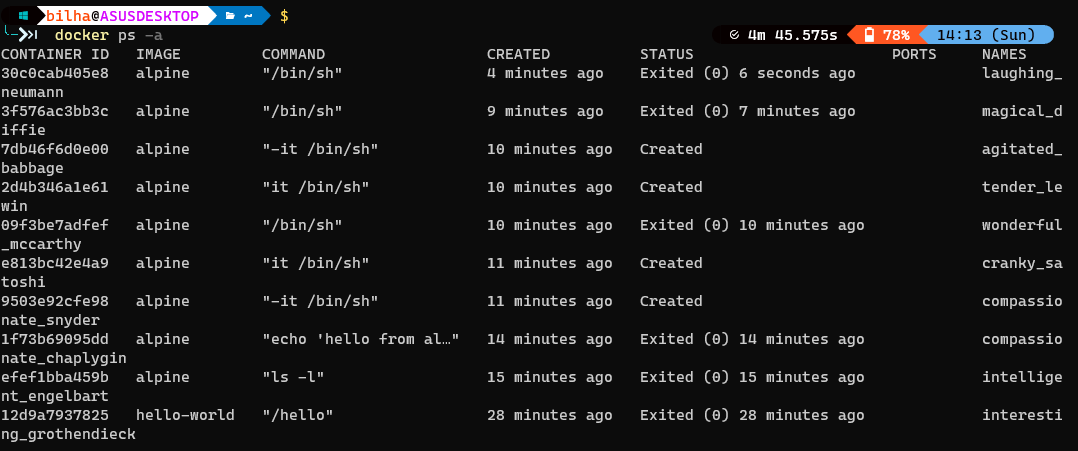
\includegraphics[width = 0.7\textwidth]{Figures/docker ps-a.png}
        \caption{Docker Ps -a}
    \end{figure}


\subsection{Apa yang terjadi ketika perintah "docker run -it" dilakukan?}
    \textit{Docker run -it} adalah sebuah \textit{command} yang memberi instruksi kepada \textit{docker} agar mengalokasi sebuah
    \textit{pseudo-TTY} atau bentuk komunikasi dua arah antara komputer utama dengan ruang yang terisolasi dengan
    membuat sebuah \textit{interactive bash shell} pada \textit{container}. 
    \begin{lstlisting}[language=bash]
        docker run -it
    \end{lstlisting}

    \begin{figure}[h]
        \centering
        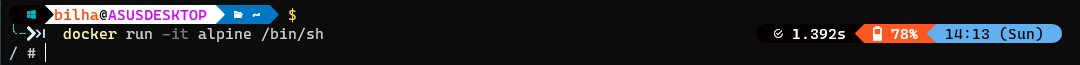
\includegraphics[width = 0.7\textwidth]{Figures/bin-sh.png}
        \caption{Docker Run -it}
    \end{figure}

\subsection{Apa yang dimaksud dengan Images?}
Docker images adalah sebuah \textit{blueprint} atau dasar dari aplikasi berbasis \textit{docker} yang memiliki sifat \textit{read-only}. Docker images sendiri 
memiliki fungsi untuk membuat \textit{docker container}, yang mana dengan satu \textit{docker images} dapat dibuat banyak \textit{docker container} \cite{hanif_2017}.

\subsection{Apa yang dimaksud dengan \textit{daemon}?}
    Daemon pada \textit{docker} adalah sebuah program yang bertugas menyelesaikan tugas di belakang layar. Daemon ini berfungsi untuk men-\textit{handling} dari \textit{docker images}, \textit{container},
    volume, dan \textit{network} di dalamnya pada \textit{request services} secara berkala ketika sistem komputer menerima sebuah perintah. Selanjutnya \textit{request} tersebut di \textit{forward} menuju 
    program lain yang umumnya berjalan di latar belakang \cite{contributor_2005}.

\newpage
\section{Kesimpulan}
    Pada tugas Hands On 3 ini dapat kami simpulkan bahwa \textit{Docker} merupakan aplikasi yang berfungsi dalam mempermudah seorang \textit{developer} dalam melakukan 
    \textit{build}, \textit{shipping}, dan \textit{run} aplikasi pada dengan sebuah \textit{container} melalui infrastruktur dari PC \textit{developer} tersebut. 
    Dengan demikian, \textit{resource} yang diperlukan dalam pembuatan suatu aplikasi hanya sedikit saja dan itu mempermudah \textit{developer}. 

		

\section{Link GitHub}
	Link GitHub dari Hands On 3 ini : \href{https://github.com/BilhaqAD07/Sistem-Operasi.git}{Klik disini}


\newpage
\bibliographystyle{IEEEtran}
\bibliography{Referensi}
\end{document}